\documentclass[11pt,usenames,dvipsnames]{beamer}
\usetheme{metropolis}

%\usepackage[utf8]{inputenc}
%\usepackage[T1]{fontenc}
\usepackage{amsmath}
\usepackage{amsfonts}
\usepackage{amssymb}
\usepackage{graphicx}
%\usepackage[MeX]{polski}
\usepackage{fancybox}
\usepackage[normalem]{ulem}
\usepackage{ucs}
\usepackage{tikz}
\usepackage{listings}
\usepackage{fancyvrb}
\usepackage{setspace}
\usepackage{silence}
\usetikzlibrary{shapes,arrows, positioning}
\lstset{%
  language = python,
  basicstyle=\scriptsize\ttfamily,
  tabsize=2,
  morekeywords={},
  moredelim=*[s][\ttfamily]{:}{:},
  keywordstyle={\bfseries\color{Blue}},
  inputencoding=utf8x,
  extendedchars=\true,    
  literate={ą}{{\k{a}}}1
  {Ą}{{\k{A}}}1
  {ę}{{\k{e}}}1
  {Ę}{{\k{E}}}1
  {ó}{{\'o}}1
  {Ó}{{\'O}}1
  {ś}{{\'s}}1
  {Ś}{{\'S}}1
  {ł}{{\l{}}}1
  {Ł}{{\L{}}}1
  {ż}{{\.z}}1
  {Ż}{{\.Z}}1
  {ź}{{\'z}}1
  {Ź}{{\'Z}}1
  {ć}{{\'c}}1
  {Ć}{{\'C}}1
  {ń}{{\'n}}1
  {Ń}{{\'N}}1
}
\lstset{breaklines=true, breakatwhitespace=true}
\author{Grzegorz Bokota}
\title{PyQt5 – introduction}
%\subtitle{}
%\logo{}
%\institute{}
%\date{}
%\subject{}
%\setbeamercovered{transparent}
%\setbeamertemplate{navigation symbols}{}
\newenvironment{CVerbatim}
{\singlespacing\center\BVerbatim}
{\endBVerbatim\endcenter}
\makeatletter
\newenvironment{CenteredBox}{\begin{Sbox}}{\end{Sbox}\centerline{\parbox{\wd\@Sbox}{\TheSbox}}}% And output it centered
\makeatother

\WarningFilter{latex}{Overwriting}
\WarningFilter{latexfont}{LaTeX Font Warning}
\WarningFilter{latex}{LaTeX Font Warning}
\WarningFilter{latexfont}{Font shape}
\WarningFilter{latexfont}{Some font}
\WarningFilter{latexfont}{Size substitutions}
\begin{document}
\begin{frame}[plain]
  \maketitle
\end{frame}
\section{Event-driven programming}
\begin{frame}{Event-driven programming – overview}
  This is programming paradigm where programmer do not control data flow 
  in program. Person, who wrote program prepare solution for every 
  event which should be handle.

  Main application: 
  \begin{itemize}
    \item GUI
    \item Network programming (server client architecture) 
  \end{itemize}
  From some point of view Object programming is version off Event-driven programing 
\end{frame}
\section{PyQt5 – base information}
\begin{frame}{Qt}
  \begin{itemize}
    \item Set of multiplatform libraries
    \item Gain access for component for creating GUI, server and console applications
    \item Wrote in C++
    \item Has bindings in other languages 
    \item Current version: 5
    \item Free (GPL, LGPL) for non commercial use. 
  \end{itemize} 
\end{frame}
\begin{frame}[c]{PyQt}
  \begin{itemize}
    \item Available under GNU GPL v3 and Riverbank Commercial License (More restrictive than Qt)
    \item There are version for Qt4 and Qt5 (strong suggest for Qt5 version)
    \item It is integrated with matplotlib plot engine
    \item Mainly use python builtin types.
    \item It is easy to use Qt documentation during use PyQt. 
  \end{itemize}
\end{frame}
\begin{frame}{`Event` type}
  \begin{description}
    \item[Event] – interaction connected with this object:
      \begin{itemize}
        \item Window show, close, resize, \dots
        \item Mouse move
      \end{itemize}
    \item[Signal] – some event happen for other object:
      \begin{itemize}
        \item Button clicked 
        \item Item selected 
        \item \textbf{Custom signal}
      \end{itemize}
  \end{description}
  
\end{frame}
\section{Introduction to PyQt programing}
\begin{frame}[fragile, c]{QApplication}
  Main class needed for execute application. 
  It contains \emph{mainloop} which looks for events 
  and execute functions connected with this events

  Simplest run:
  \begin{lstlisting}
  myApp = QApplication(sys.argv)
  wind = MainWindow(...) # custom class
  wind.show()
  myApp.exec_()
  \end{lstlisting}
\end{frame}
\begin{frame}[fragile, c]{QMainWindow}
  Base class suggested for application main window. 
  Add place for main menu and statusbar 
  \begin{figure}[htpb]
  \begin{center}
    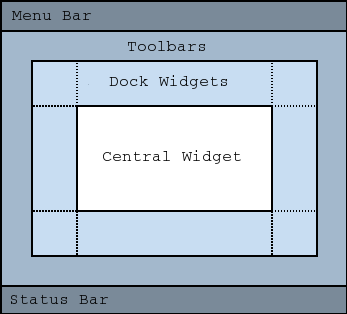
\includegraphics[width=0.5\linewidth]{./mainwindowlayout.png}
  \end{center}
  \caption{QMainWindow}\label{fig:mainwindow}
  \end{figure}  
\end{frame}
\begin{frame}[c]{QDialog}
  Class for all dialog windows.
  Dialog window block all other windows until is active.

  \begin{itemize}
    \item QFileDialog
    \item QInputDialog
    \item QMessageBox
    \item \dots
  \end{itemize}
  \begin{figure}[htpb]
    \centering
    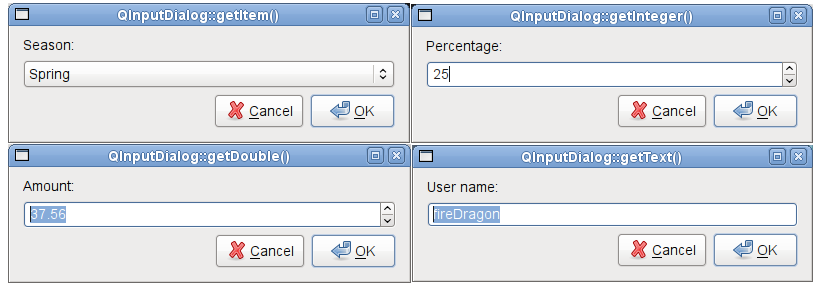
\includegraphics[width=0.8\linewidth]{./inputdialogs.png}
    \caption{QInputDialog}
    \label{fig:input}
  \end{figure}
  
\end{frame}
\begin{frame}[c]{Other}
  \begin{itemize}
    \item QWidget – Base for all other
    \item QPushButton
    \item QCheckBox 
    \item QTableWidget
    \item QProgressBar
    \item QLineEdit
    \item QSpinBox
    \item QLabel – text can be formatted with simple HTML
  \end{itemize}
\end{frame}
\begin{frame}[fragile,c]{Layout}
  Of course we can set position of each element manually using \lstinline|ob.move(const QPoint&)|. 
  But in this case we need update it manually after each change. Easier would be if framework will do it for us.  
  \begin{itemize}
    \item QGridLayout
    \item QHBoxLayout
    \item QVBoxLayout 
  \end{itemize}
\begin{lstlisting}
main_layout = QVBoxLayout()
btn_lay = QHBoxLayout()
btn_lay.addWidget(self.new_matrix_btn)
btn_lay.addWidget(self.save_btn)
btn_lay.addWidget(self.load_btn)
main_layout.addLayout(btn_lay)
\end{lstlisting}
\end{frame}
\begin{frame}[fragile,c]{Matplotlib integration}
  Import:
  \begin{lstlisting}
from matplotlib.backends.backend_qt5agg import FigureCanvasQTAgg as FigureCanvas
  \end{lstlisting}
  Usage:
  \begin{lstlisting}
fig = pyplot.figure(figsize=(6, 6), dpi=100, frameon=False, facecolor='1.0', edgecolor='w', tight_layout=True)
self.figure_canvas = FigureCanvas(fig)
self.fig_num = fig.number
  \end{lstlisting}
  Reuse:
  \begin{lstlisting}
fig = pyplot.figure(self.fig_num)
pyplot.imshow(self.matrix, cmap=self.cmap)
fig.canvas.draw()
  \end{lstlisting}
\end{frame}
\section{Tasks}
\begin{frame}[c]{Tasks}
  \begin{enumerate}
    \item Add colormap choose with \lstinline|QComboBox|
    \item Add checkbox which allow break symmetry  
  \end{enumerate}
\end{frame}
\end{document}

